\chapter{Längenmetriken}

\section{Graphen --- Definitionen}

\begin{definition}{Graph}
  Ein \emph{Graph} $ G = (E, K) $ besteht aus einer \emph{Ecken}-Menge $ E $ und einer Menge von Paaren $ \{ u, v \} $ ($ u, v \in E $), genannt \emph{Kanten}.
\end{definition}

\begin{marginfigure}
    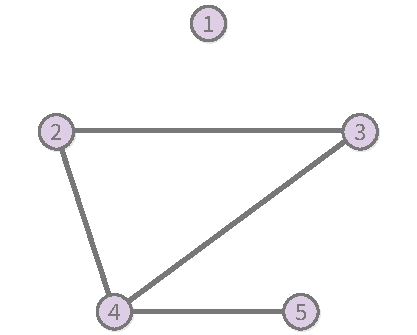
\includegraphics[width=\linewidth]{2017-10-18-03}
    \caption{Ein einfacher Graph. Dieser Graph ist \underline{nicht} zusammenhängend, da die Ecke $ 1 $ nicht von den anderen Ecken aus erreicht werden kann.}
\end{marginfigure}

\begin{definition}{Erreichbarkeit}
  Seien $ p, q \in E $ von $ G = (E, K) $. $ q $ ist \emph{erreichbar} von $ p $ aus, falls ein \emph{Kantenzug} von $ p $ nach $ q $ existiert.
\end{definition}

\begin{definition}{Zusammenhängend}
  $ G = (E, K) $ heißt \emph{zusammenhängend}, falls alle Ecken von einer beliebigen, festen Ecke aus erreichbar sind.
  \\ \ \\
  Ist $ G $ ein zusammenhängender Graph, so ist $ d(p, q) = $ minimale Kantenzahl eines Kantenzuges von $ p $ nach $ q $ eine Metrik.
\end{definition}